\documentclass[a4paper,
fontsize=11pt,
%headings=small,
oneside,
numbers=noperiodatend,
parskip=half-,
bibliography=totoc,
final
]{scrartcl}

\usepackage{synttree}
\usepackage{graphicx}
\setkeys{Gin}{width=.9\textwidth} %default pics size

\graphicspath{{./plots/}}
\usepackage[ngerman]{babel}
\usepackage[T1]{fontenc}
%\usepackage{amsmath}
\usepackage[utf8x]{inputenc}
\usepackage [hyphens]{url}
\usepackage{booktabs} 
\usepackage[left=2.4cm,right=2.4cm,top=2.3cm,bottom=2cm,includeheadfoot]{geometry}
\usepackage{eurosym}
\usepackage{multirow}
\usepackage[ngerman]{varioref}
\setcapindent{1em}
\renewcommand{\labelitemi}{--}
\usepackage{paralist}
\usepackage{pdfpages}
\usepackage{lscape}
\usepackage{float}
\usepackage{acronym}
\usepackage{eurosym}
\usepackage[babel]{csquotes}
\usepackage{longtable,lscape}
\usepackage{mathpazo}
\usepackage[normalem]{ulem} %emphasize weiterhin kursiv
\usepackage[flushmargin,ragged]{footmisc} % left align footnote
\usepackage{ccicons} 
\setcapindent{0pt} % no indentation in captions

%%%% fancy LIBREAS URL color 
\usepackage{xcolor}
\definecolor{libreas}{RGB}{112,0,0}

\usepackage{listings}

\urlstyle{same}  % don't use monospace font for urls

\usepackage[fleqn]{amsmath}

%adjust fontsize for part

\usepackage{sectsty}
\partfont{\large}

%Das BibTeX-Zeichen mit \BibTeX setzen:
\def\symbol#1{\char #1\relax}
\def\bsl{{\tt\symbol{'134}}}
\def\BibTeX{{\rm B\kern-.05em{\sc i\kern-.025em b}\kern-.08em
    T\kern-.1667em\lower.7ex\hbox{E}\kern-.125emX}}

\usepackage{fancyhdr}
\fancyhf{}
\pagestyle{fancyplain}
\fancyhead[R]{\thepage}

% make sure bookmarks are created eventough sections are not numbered!
% uncommend if sections are numbered (bookmarks created by default)
\makeatletter
\renewcommand\@seccntformat[1]{}
\makeatother


\usepackage{hyperxmp}
\usepackage[colorlinks, linkcolor=black,citecolor=black, urlcolor=libreas,
breaklinks= true,bookmarks=true,bookmarksopen=true]{hyperref}
\usepackage{breakurl}

%meta
\expandafter\def\expandafter\UrlBreaks\expandafter{\UrlBreaks%  save the current one
  \do\a\do\b\do\c\do\d\do\e\do\f\do\g\do\h\do\i\do\j%
  \do\k\do\l\do\m\do\n\do\o\do\p\do\q\do\r\do\s\do\t%
  \do\u\do\v\do\w\do\x\do\y\do\z\do\A\do\B\do\C\do\D%
  \do\E\do\F\do\G\do\H\do\I\do\J\do\K\do\L\do\M\do\N%
  \do\O\do\P\do\Q\do\R\do\S\do\T\do\U\do\V\do\W\do\X%
  \do\Y\do\Z}
%meta

\fancyhead[L]{Chr. Meskó\\ %author
LIBREAS. Library Ideas, 35 (2019). % journal, issue, volume.
\href{http://nbn-resolving.de/}
{}} % urn 
% recommended use
%\href{http://nbn-resolving.de/}{\color{black}{urn:nbn:de...}}
\fancyhead[R]{\thepage} %page number
\fancyfoot[L] {\ccLogo \ccAttribution\ \href{https://creativecommons.org/licenses/by/4.0/}{\color{black}Creative Commons BY 4.0}}  %licence
\fancyfoot[R] {ISSN: 1860-7950}

\title{\LARGE{Die Torwächter des öffentlichen Wissens \\ Politischer Positionsbezug gegen rechts von Öffentlichen Bibliotheken in Deutschland}}% title
\author{Christian Meskó} % author

\setcounter{page}{1}

\hypersetup{%
      pdftitle={Die Torwächter des öffentlichen Wissens. Politischer Positionsbezug gegen rechts von Öffentlichen Bibliotheken in Deutschland},
      pdfauthor={Christian Meskó},
      pdfcopyright={CC BY 4.0 International},
      pdfsubject={LIBREAS. Library Ideas, 35 (2019).},
      pdfkeywords={Inklusion, Politik für Alle, Politikbibliothekarische Arbeit, Rassismus, Bestandserweiterung, Fachpersonal, diversity management, transkulturelle Arbeit},
      pdflicenseurl={https://creativecommons.org/licenses/by/4.0/},
      pdfcontacturl={http://libreas.eu},
      baseurl={http://libreas.eu},
      pdflang={de},
      pdfmetalang={de}
     }



\date{}
\begin{document}

\maketitle
\thispagestyle{fancyplain} 

%abstracts
\begin{abstract}
Gegenwärtig erlebt der Rückbezug auf vermeintlich bedrohte nationale und
kulturelle Identitäten weltweit einen Aufschwung. Ursachen dafür werden
oft in den, durch zahlreiche Kriegs- und Konfliktherde ausgelösten,
Bewegungen von Flüchtlingen ausgemacht, die es in das Zentrum
kapitalistischer Wohlfahrtsstaaten zieht. Die Instrumentalisierung von
Abstiegsängsten bei den Mittel- und Unterschichten betroffener Länder,
wird aber nicht nur auf den digitalen Plattformen sozialer Medien
betrieben, sondern auch auf den etablierten Podien und in den
traditionellen Institutionen öffentlicher Wissensvermittlung. Die
rechtsnationalen bis rechtsradikalen Stimmen inszenieren sich
gegenwärtig oft als Opfer, weil sie angeblich nicht mehr gehört würden.
Sie empören sich in diesem Zusammenhang, weil Sie eine angebliche
Mehrheitsmeinung aussprechen, die vermeintlich lange genug durch
liberale Wortkosmetik tabuisiert wurde. Durch immer professionellere
Medienstrategien haben sie aber längst erreicht, dass ihre Stimmen im
Gegenteil unverhältnismäßig oft gehört und medial verbreitet werden. Zu
den Bühnen, die sie wählen, gehören Zeitungen, soziale Netzwerke,
Talkshows, Podiumsdiskussionen und Demonstrationen ebenso, wie etwa die
Bestände von Buchhandlungen und Bibliotheken. Im Spannungsfeld von
Neutralität, Informationsfreiheit und den Schutzrechten diskriminierter
Minderheiten, stellt sich auch dem Fachpersonal öffentlicher
Bibliotheken die Frage, wie sie die Öffentlichkeit darin unterstützen
kann, die Debatten nicht von Rechtsnationalen und Rechtsextremen
vereinnahmen zu lassen. Ohne Zensur auszuüben oder für bestimmte Gruppen
Partei zu ergreifen, hat das Fachpersonal von öffentlichen Bibliotheken
die schwierige Herausforderung zu bewältigen, darauf eine Antwort zu
finden.
\end{abstract}

%body
\hypertarget{einleitung}{%
\section*{Einleitung}\label{einleitung}}

Warum können rechtsnationalistische bis offen rechtsextreme Parteien in
ganz Europa und auch international so eindeutige Wahlgewinne aufweisen?
Wieso gelingt es den etablierten politischen Kräften und öffentlichen
Verwaltungen so wenig argumentativ überzeugende Antworten zu geben und
intelligente Debattenformate zu organisieren, um auf die immer massivere
Kritik von rechten Gruppen an offenen Gesellschaften zu reagieren? Eine
Antwort auf diese, zugegebenermaßen recht komplexen, Fragestellungen,
könnte darauf verweisen, dass die Schere zwischen arm und reich global
noch nie so weit auseinander klaffte wie gegenwärtig (Piketty, 2016,
S.~31--33, 39--41 und 573--624). Die Wut derjenigen, die sich im
kapitalistischen Wettbewerb von den Eliten gesellschaftlicher
Entscheidungsfindung allein gelassen fühlen, so könnte man
argumentieren, wird geschickt instrumentalisiert und auf Flüchtlinge,
Fremde und ausländische Arbeitsuchende projiziert. So stellt
beispielsweise auch die Wochenzeitschrift die Zeit fest:

\begin{quote}
Auch im siebten Jahr nach Ausbruch der Finanz- und Wirtschaftskrise
herrscht in der großen Masse der Bevölkerung das Gefühl, dass die
Reichen \enquote{es sich richten können} und mit ihren Vermögen auch
ihren politischen Einfluss über Generationen weiterreichen (Rehm \&
Schnetzer, 2015, Abschnitt 9).
\end{quote}

Für das Selbstbild und die politische Positionierung öffentlicher
Bibliotheken ist allerdings nicht die Engführung von Antworten auf
komplexe Fragestellungen zu suchen, sondern die Kompetenz gerade solche
komplexen gesellschaftspolitisch umkämpften Themenbereiche und
gesellschaftlich relevanten Debatten und Diskurse aus möglichst vielen
Quellen abzubilden, zu kommentieren und vor dem Hintergrund einer
faktenbasierten Recherche einzuordnen.

\hypertarget{bibliotheken-als-neutraler-vermittlungsort-fuxfcr-information-und-von-diskursen-und-debatten}{%
\section*{Bibliotheken als neutraler Vermittlungsort für
Information und von Diskursen und
Debatten?}\label{bibliotheken-als-neutraler-vermittlungsort-fuxfcr-information-und-von-diskursen-und-debatten}}

Es bleibt als Einwand nicht abzuwehren, dass öffentliche Bibliotheken
natürlich sorgsam zwischen dem Neutralitätsgebot, der
Informationsfreiheit und den Schutzrechten diskriminierter Minderheiten
abwägen müssen.

Das Neutralitätsgebot leitet sich in Deutschland unter anderem von dem
im Grundgesetz (Art. 3 I GG) verankerten Gleichheitsgrundrecht ab
(Deutschland. Bundesministerium der Justiz und für Verbraucherschutz
(o.~D.)). Aber wie können politische Botschaften, unter denen nicht die
wenigsten die Schutzrechte diskriminierter gesellschaftlicher Gruppen
bedrohen, neutral behandelt werden? Ebenso im Grundrecht verankert ist
auch die Informationsfreiheit (Art. 5 I 1 2. Var. GG), wonach
\enquote{{[}jede und{]}\footnote{Diese Ergänzung wurde vom Autor selbst
  hinzugefügt, um die Relevanz von geschlechtergerechter Sprache gerade
  auch in diesem Zusammenhang nicht zu vernachlässigen.} jeder} das
Recht haben, \enquote{sich aus allgemein zugänglichen Quellen
ungehindert zu unterrichten} (Deutschland. Bundesministerium der Justiz
und für Verbraucherschutz (o.~D.)). Wenn aber zudem die Schutzrechte
diskriminierter Minderheiten im Auge behalten werden sollen, muss in
zweifellos aufwendigen Verfahren sichergestellt werden, dass keine
verfassungsfeindlichen, rassistischen, antisemitischen oder anderweitig
diskriminierenden Inhalte ohne entsprechende Kennzeichnung,
Kommentierung und Einordnung in den Bestand aufgenommen werden. Zunächst
einmal stellt sich aber die Frage, ob sie überhaupt aufgenommen werden
sollen.

\hypertarget{kommentierte-oder-unkommentierte-aufnahme-in-den-bestand}{%
\section*{Kommentierte oder unkommentierte Aufnahme in den
Bestand?}\label{kommentierte-oder-unkommentierte-aufnahme-in-den-bestand}}

Wer sich aber inhaltlich mit den immer professioneller argumentierenden
rechtsextremen und rechtsnationalen Meinungsplattformen und deren
Galionsfiguren auseinandersetzen will, wird schnell mit dem zunächst
intuitiv nachvollziehbaren Argument konfrontiert, dass die Einschränkung
von Meinungsfreiheit zum Schutz diskriminierter Minderheiten schnell zur
Zensur werden kann. Eben dieser Zensur-Vorwurf wurde beispielsweise vom
Gemeinschafts-Blog \enquote{Die Freie Welt} des AfD-Polit-Personals
Beatrix und Sven von Storch, die bei dem Blog auch die verantwortliche
Redaktion stellen, an die öffentlichen Bibliotheken gerichtet (Die Freie
Welt, 2018, 3. Januar). Allerdings wird das nur im Titel und Übertitel
des Beitrags suggeriert, die ‚Zensur in Bibliotheken' und ‚Bücher sollen
aussortiert werden' heißen (ebd.). Liest man allerdings den ganzen
Beitrag wird schnell klar, dass es nicht die Stadt- und Landesbibliothek
Potsdam ist, der die Freie Welt den Vorwurf der Zensur macht, sondern
eher der linksalternativen Fraktion ‚DIE aNDERE' aus der
Stadtverwaltung, die sich in einer Anfrage an die Bibliothek nach
rechtsradikalen oder antisemitischen Publikationen im Bestand erkundigt
hatte (Kramer, 2017, 27. Dezember, Abschnitt 1--4). Diese Art der
absichtlich in die irre führenden Titel und Untertitel, die schon zur
Empörung führen kann, bevor der eigentlich Text gelesen wurde, ist
symptomatisch für die provokative Medienstrategie der neuen Rechten
(Herrmann, 2019, S. 156--158).

\begin{quote}
Die Andere hatte mit ihrer Anfrage prüfen wollen, ob die Zielsetzungen
des Potsdamer Aktionsplanes für Toleranz sowie Demokratie und gegen
Gewalt, Rechtsextremismus sowie Fremdenfeindlichkeit beim Literatur- und
Medienbestand der Stadtbibliothek berücksichtigt werden -- dort wird ein
generell offensiver Umgang mit rechter Propaganda empfohlen, statt diese
als Meinungsäußerung unwidersprochen zu lassen (Kramer, 2017, 27.
Dezember, Abschnitt 2).
\end{quote}

Die Bibliothek hatte hier die klare Entscheidung getroffen auch hoch
umstrittene Bestseller wie \enquote{Finis Germania -- Das Ende
Deutschlands} aus dem neurechten Verlag Antaios in ihren Bestand
aufzunehmen. Das von verschiedenen Journalisten und Historikern als
geschichtsrevisionistisch, antisemitisch und rechtsradikal kritisierte
Buch soll laut der Potsdamer Bibliotheksleiterin Marion Mattekat Teil
des Bestands der Bibliothek sein, weil auch \enquote{weltanschaulich
tendenziöse Schriften und Medieninhalte,} Relevanz haben können,
\enquote{wenn sich diese im gegenwärtigen gesellschaftlichen Diskurs
befinden} (ebd., Abschnitt 4).

Hierbei ist zu bedenken, dass viele Debatten über die Medien, die
Medienproduzenten und/oder von undurchsichtigen Gruppen oder
Einzelpersonen im Hintergrund hochgekocht, instrumentalisiert und den
eigenen Interessen entsprechend provokativ in Szene gesetzt werden.
Schon allein deshalb kann eine unkommentierte Aufnahme in den Bestand
mit dem alleinigen Verweis auf Bestseller-Listenplätze, keinesfalls
akzeptiert werden. Zum einen, weil Bestseller-Listen das
gesellschaftliche Informations- und Lese-Bedürfnis, wenn überhaupt, nur
höchst unvollkommen und verzerrt widerspiegeln. Vor allen Dingen aber,
weil man davon ausgehen muss, dass die Schutzrechte gleich mehrerer
Gruppen diskriminierter Minderheiten in solchen und vergleichbaren
neurechten Publikationen auf zahlreichen persönlichen und
gesellschaftlichen Ebenen mit Füßen getreten werden. Über das
Verlagsprogramm von Antaios\footnote{Antaios war ein Riese aus der
  griechischen Mythologie und der Sohn von Poseidon und Gaia, der Göttin
  der Erde, die ihm auch seine unbezwingbare Stärke verlieh. Antaios,
  der alle vorbeikommenden Reisenden zwang, mit ihm zu kämpfen und aus
  ihren Schädeln einen Tempel zu Ehren Poseidons fertigte und zudem
  Fremde jagte und Löwen verspeiste (Wikipedia, 2018), entspricht der
  Selbstdarstellungsstrategie der neuen Rechten, provokative,
  hypermaskuline und politisch inkorrekte Rollenvorbilder zu wählen. Da
  Antaios seine Kraft aus der Erde bezog, hat Herkules, der ihn zunächst
  nicht bezwingen konnte, ihn dann übrigens einfach in die Luft gehoben
  und erwürgt (ebd.).} und die Gedankenwelt des Verlegers Kubitschek,
berichten etwa der Geograf und Populismusforscher Alexander Reid Ross
und die Historikerin Patricia Zhubi (2019, 24. März, Abschnitt 4) in
einem Überblicksartikel über die globale Ideologie und Medienstrategien
rechtsterroristischer Netzwerke nach dem Christchurch-Attentat in
Neuseeland.

\begin{quote}
Der neurechte Verleger Götz Kubitschek wünscht sich die Krise herbei,
sie sei dem \enquote{Rückfall ins Siechtum, ins Latente, ins Erdulden}
vorzuziehen. \enquote{Ein solcher Antirationalismus mündet zwangsläufig
in der Glorifizierung von Gewalt}, so der Hamburger Historiker Volker
Weiß. Hiervon zeuge das Buch \emph{Der Weg der Männer} des
US-amerikanischen Alt-Right-Autors Jack Donovan, das bei Kubitscheks
Verlag Antaios publiziert wurde. Ewiger Friede ist laut Donovan der
\enquote{Tod der Männlichkeit}, eine Überzeugung, die auch der
Christchurch-Attentäter teilt (ebd.).
\end{quote}

Es darf kein Zweifel daran bestehen, dass das Fachpersonal von
öffentlichen Bibliotheken die Verbreitung von solcherlei
menschenfeindlichem Gedankengut nicht zulassen darf. Die Frage ist nur,
wie die Verbreitung verhindert werden kann. Falls dann die Entscheidung
hinsichtlich einer kommentierten und in entsprechende Verschlagwortungen
und Kategorien eingeordneten Aufnahmen in den Bestand erfolgt, stellt
sich zudem die Frage wie und von wem diese Einordnungen vorgenommen
werden sollten.

\hypertarget{gegen-eine-aufnahme-von-rechten-publikationen-in-bibliotheken-und-buchhandlungen}{%
\section*{Gegen eine Aufnahme von rechten Publikationen in
Bibliotheken und
Buchhandlungen?}\label{gegen-eine-aufnahme-von-rechten-publikationen-in-bibliotheken-und-buchhandlungen}}

Jörg Sundermaier vom Verbrecher Verlag in Berlin argumentiert
beispielsweise gegen eine Aufnahme von rechten Verlagen und
Publikationen in das Sortiment von Buchhandlungen und Bibliotheken und
begründet dies, unter anderem, mit der Taktik von rechten Gruppen und
Einzelpersonen, mit wiederholten Nachfragen in Buchhandlungen und
Bibliotheken auf das Anschaffen bestimmter Publikationen zu drängen
(Sundermaier, 2018, S. ~332--333 und Baeck, 2018, 21. November). Es ist
natürlich keineswegs illegitim seine Meinung und Wünsche in Bezug auf
den Bestand von Bibliotheken und Buchhandlungen zum Ausdruck zu bringen.
Auch dann nicht, wenn man die Publikationen selbst schon kennt und
vielmehr dafür sorgen möchte, dass die eigenen politischen Vorstellungen
weiterverbreitet werden (Sundermaier, 2018, S. ~332--333). Allerdings
müssen Bibliotheken und auch Buchhandlungen im Auge behalten, dass nicht
nur interessierte Einzelpersonen, sondern eben auch effizient
organisierte Netzwerke rechtsextremer Gruppen (Stöss, 2000, S. 6--21 und
Hübner, 2008, S. 17--18) und Denkfabriken aus strategischen Gründen
immer wieder die gleichen Sympathisanten an bestimmte Stellen senden
könnten, immer mit dem Vorwurf im Handgepäck, bestimmte Themenbereiche
würden ausgegrenzt, tabuisiert und totgeschwiegen. Schickt man nur eine
Handvoll Leute (mit genug Zeit) über einen Monat verteilt in eine
bestimmte Bibliothek oder Buchhandlung und lässt dieselben Leute auch
E-Mails schreiben und anrufen, kann für eine Stadtteilbibliothek oder
eine regionale Buchhandlung schnell der Eindruck entstehen, dass genau
die nachgefragten Publikationen gerade sehr viel Interesse wecken. Um
den Überblick über solche Formen der Beeinflussung verschiedener
Meinungsfronten zu behalten, forderte bereits Boryano Rickum in seinem
Essay \enquote{Politikbibliothekarische Arbeit}, das Bibliothekspersonal
unter anderem den Überblick über tagesaktuelle und grundsätzliche
politische Debatten lokal und weltweit im Blick behalten muss (Rickum,
2017, S. 630). Zudem erwähnt Sundermeier als weitere Argumente gegen
eine Aufnahme von rechter Literatur in den Bestand von Buchhandlungen
und Bibliotheken, schlecht recherchierte und argumentierte
Verschwörungstheorien und die oft miserable Qualität der Editionen
(Sundermaier, S. 333).

Es muss allerdings klar und offen kommuniziert werden, dass einerseits
niemand politische Wahrheit für seine Position oder politische
Überzeugung in Anspruch nehmen kann und andererseits längst anerkannte
Tatsachen, wie etwa der Holocaust oder die Kugel-Form der Erde, nicht
ernsthaft erneut in Frage gestellt werden können. Zumindest nicht in
Archiven der öffentlichen Wissensvermittlung und ohne jegliche
Kommentierung oder Einordnung. Natürlich wird es, gerade in dem aktuell
polarisierten gesellschaftspolitischen Klima, besonders schwierig diese
Einordnungen, Kommentierungen und kategorischen Etikettierungen
vorzunehmen.

Dem Einen wird etwa Sarrazins (2010) \enquote{Deutschland schafft sich
ab} nur das professorale Konvolut eines beherzten Konservativen
innerhalb der SPD sein, der möglicherweise etwas unbedacht
biologistische Argumentationen mit ethnisch-kulturellen Statistiken in
Zusammenhang bringt. Dem Anderen ist er die Speerspitze nie wirklich
reflektierten nationalsozialistischen Gedankenguts in der
bürgerlich-akademischen Mittelschicht. Zwischen diesen Polen müssen
Bibliotheken und ihr ausgebildetes Fachpersonal vermitteln und wenn
möglich Dialoge zwischen verhärteten Fronten fördern. Aber vor allen
Dingen müssen Sie die Netzwerke, Hintergründe und Etymologien dieser
Gedankenwelten kennen, um sie wirklich Einordnen und als Bibliothek zu
diesen Positionen Stellung beziehen zu können.

\hypertarget{eindeutige-einordnung-und-kommentierung-von-rassistischer-oder-anderweitig-diskriminierender-literatur}{%
\section*{Eindeutige Einordnung und Kommentierung von rassistischer
oder anderweitig diskriminierender
Literatur}\label{eindeutige-einordnung-und-kommentierung-von-rassistischer-oder-anderweitig-diskriminierender-literatur}}

Der Autor des vorliegenden Essays hätte persönlich wenig dagegen
einzuwenden, wenn rechte Publikationen, wie Sarrazins Machwerk gar nicht
mehr in Bibliotheken auftauchen. Wenn aber der Entschluss für eine
Aufnahme in den Bestand erfolgt, gehört zur Minimalanforderung an eine
kompetente Einordnung, dass der Publikation kritische Erkenntnisse, wie
etwa die der Forschergruppe um die Wissenschaftlerin Dr.~Naika Foroutan
von der Humboldt-Universität, zur Seite gestellt werden, die am Ende der
Publikation \enquote{Sarrazins Thesen auf dem Prüfstand} (2011, S. 57)
anmerkt:

\begin{quote}
Dieses Dossier befasst sich mit Thilo Sarrazins Thesen zur Integration
von Muslimen in Deutschland, die er in seinem Buch \enquote{Deutschland
schafft sich ab} (Wiesbaden 2010, 1. Auflage) aufgestellt hat. Es ist
eine empirische Gegenüberstellung, die einen ersten Überblick darüber
geben soll, wie die in dem Buch verwendeten Zahlen zu Zuwanderung und
Integration auf Grundlage desselben Datenmaterials und ergänzenden
wissenschaftlichen Studien unterschiedlich gewertet werden können. Das
Dossier soll als ein erster Impuls verstanden werden, der einen Zugang
zu den vielzähligen wissenschaftlichen Studien zum Themenfeld
Integration und Muslime in Deutschland eröffnen und zu vertiefenden
Analysen anregen soll.
\end{quote}

Zudem werden die Autoren in einer Publikation der Bundeszentrale für
politische Bildung (2011) zum gesellschaftlichen Einfluss von Sarrazins
Thesen folgendermaßen zitiert:

\begin{quote}
Als \enquote{tendenziös und pauschal abwertend} beurteilen die Autoren
Sarrazins Thesen. Das \enquote{gezielte Verschweigen} einer weitgehend
erfolgreichen Integration und die \enquote{Ausweitung des Diskursraums
bis an die Grenzen der Diffamierung} drohen die zuvor messbaren
Integrationserfolge rückgängig zu machen. Nicht Integration, sondern
\enquote{Ängste, Ressentiments und rassistische Abwehrreaktionen} seien
in der Auseinandersetzung mit seinen Thesen verhandelt worden, schreiben
die Autoren (Abschnitt 10).
\end{quote}

Darüber hinaus, vor allen Dingen auch weil es für viele Menschen schon
zu lange dauert solche Aussagen ganz zu lesen, muss der Text eindeutig
in irgendeiner Form in der Kategorie rassistische bis stark
diskriminierende Literatur eingeordnet werden. So eingebettet und auch
rein physisch, auf dem entsprechenden bibliothekarischen Bücherregal von
kritischen Gegenargumenten umgeben, könnten auch solche Texte nicht nur
von Forschenden der Sozialwissenschaften, sondern auch von Laien klarer
verortet werden, als wenn das Buch unkommentiert zwischen alle anderen
Sachbuch-Bestseller gestellt wird.

\hypertarget{gegen-rassistische-und-diskriminierende-verschlagwortung-und-kategorisierungen-in-bibliotheken}{%
\section*{Gegen rassistische und diskriminierende Verschlagwortung
und Kategorisierungen in
Bibliotheken}\label{gegen-rassistische-und-diskriminierende-verschlagwortung-und-kategorisierungen-in-bibliotheken}}

Aber damit nicht genug. Das Fachpersonal in öffentlichen Bibliotheken
müsste sowohl in den Katalogisierungs- und Indexierungssystemen, als
auch in den thematischen Kategorien der eigenen Bibliothek sensibel, und
im vollen Bewusstsein der polarisierten gesellschaftlichen Meinungen,
jede diskriminierende Einordnung vermeiden, auflösen oder entsprechend
kommentieren. Natürlich würden dafür unabhängige Kollektive
interdisziplinär aufgestellter Teams von Fachpersonal mit sozial-,
kommunikations-, geschichts-, kultur- und informationswissenschaftlichem
Hintergrundwissen benötigt. Sie sollten beispielsweise verhindern
helfen, dass bei dem Musik-Streamingdienst \enquote{Freegal} der
öffentlichen Bibliotheken Berlins ein rassistisches Kinderlied angezeigt
wird (das in den Archiven gar nicht verfügbar sein dürfte), wenn man in
das Suchfeld \enquote{zehn kleine\ldots{}} eingibt und die Vorschläge,
die das System macht, das letzte Wort nicht nur mit
\enquote{Zappelmänner(n)}, sondern an vierter Stelle, nach
\enquote{Fröschlein} und \enquote{Zappelfinger}, mit dem rassistischen
N-Wort vervollständigt.

\begin{figure}
\centering
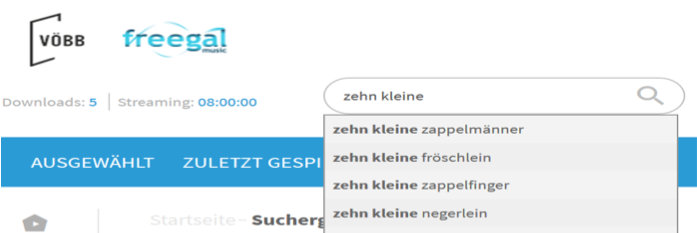
\includegraphics{abb_1.png}
\caption{Screenshot von den Vorschlägen des Freitext-Suchfelds des
Musik-Streamingdienstes \enquote{Freegal} des Verbundes der öffentlichen
Bibliotheken Berlins (VÖBB). 28.08.2019. 15:14. Abgerufen von
\url{https://voebb.freegalmusic.com/search-page/zehn\%2520kleine\%2520negerlein}}
\end{figure}

Auch ewig wiederkehrende Empörungsquellen, wie das Comic \enquote{Tim im
Kongo} wegen eindeutig kolonialistischer und rassistischer Stereotype
ohne jegliche historische und kolonialismus-kritische Analyse und
Einordnung keinesfalls in den Bestand von Kinder- und Jugendbibliotheken
gehört, sind erneut und weiterhin klar zu benennen.

\begin{quote}
Im zweiten Band \emph{Tim im Kongo} (\emph{Tintin au Congo}, 1931) sind
\enquote{Rassismus und Kolonialismus {[}\ldots{}{]} so offensichtlich,
dass es da nichts nachzuweisen oder zu überführen gibt} (Seeslen, 2011,
S. 81 zitiert nach Planka, 2012, S.241).
\end{quote}

Dennoch hat der Autor dieses Essays bislang weder in Berlin noch in
anderen deutschen Städten in Kinder- und Jugendbibliotheken eine solche
kritische Kommentierung gefunden. Den rassistischen Comic konnte man
dagegen fast überall ausleihen.

Diese hoffentlich eindrücklichen Alltags-Beispiele, könnten mit ihren
folgenreichen Forderungen auch wieder schnell als Zensur angegriffen
werden. Darüber hinaus hätten sicherlich einige als Gegenargument
vorzubringen, dass gerade der hyperkorrekte politische Röntgenblick
einer akademischen Elite von Kultur- und Sozialwissenschaftlern normale
Menschen so sehr genervt hat, dass sie dann, schon aus Protest, lieber
AfD und andere rechtsextreme Gruppen gewählt oder diese in anderer Form
unterstützt haben. Im selben Fahrwasser könnte man argumentieren, dass
eine freiheitlich demokratische Gesellschaft auf so vielen Ebenen
bedroht wird, dass es völlig unverhältnismäßig ist, sich mit
rassistischen Wörtern und Bedeutungszusammenhängen in Kinderliedern und
Comics zu beschäftigen.

Dem muss entschieden widersprochen werden. Koloniales, rassistisches und
jegliche Gruppen von Minderheiten diskriminierendes Gedankengut ist so
tief und seit so vielen Generationen in allen Kulturtechniken
menschlicher Politik, Wirtschaft, der Wissenschaft, Kunst und Kultur
reproduziert worden, dass jeder noch so unbedeutende wirkende Faden
dieses Teppichs auseinandergenommen genommen werden muss; von
Kinderbüchern bis zu Image-Filmen auf YouTube; von Bilderserien auf
Instagram bis zu dem Twitter-Feed des amerikanischen Präsidenten; von
Bestsellern, die vermeintliche, aber gar nicht vorhandene Sprechverbote
adressieren bis zu dem selbst gefilmten und auf Facebook gestreamten
Live-Feed des Christchurch Attentäters, der sich in seinem eigenen
Manifest auf das des Massenmörders Breivik bezogen hat. Alles muss
analysiert, eingeordnet und in seiner Gefährlichkeit für ein
empathisches und gewaltfreies gesellschaftliches Zusammenleben benannt
werden. Nicht die Mikro-Konfliktfelder sollten dabei im Fokus sein,
sondern die Medien- und Propagandastrategien rechter Netzwerke, die
antirassistische, feministische, gegen Gewalt und für Toleranz
eintretende Kräfte insgesamt angreifen und ihre Bemühungen einer
globalen liberal-kapitalistischen Elite vorwerfen. Es ist nicht von der
Hand zu weisen, dass diese Elite tatsächlich in hohem Maß zur
Polarisierung der Gesellschaft beigetragen hat. Tragisch und
gleichermaßen unhaltbar wäre in diesem Zusammenhang allerdings, wenn wir
alle ohnmächtig den Nebelkerzen rechter Propaganda zusehen, wie sie
linke Globalisierungskritik kapern, mit Kulturprotektionismus und
identitärer Ideologie vermischen und statt die verantwortlichen
politischen und wirtschaftlichen Eliten schon wieder Minderheiten
verantwortlich machen, die am meisten unter den gegenwärtigen Krisen
leiden.

\hypertarget{fuxfcnf-vor-zwuxf6lf}{%
\section*{Fünf vor Zwölf}\label{fuxfcnf-vor-zwuxf6lf}}

Um dem entgegenzuwirken und den provokativen und mittlerweile sehr
professionellen Medienstrategien rechtsextremer Netzwerke und
lautstarker Einzelpersonen argumentativ und mit einer konsistenten
Gesamtstrategie zu begegnen, wäre ein erster großer Schritt getan, wenn
die Gefahr, die von ihnen ausgeht, zunächst einmal wirklich anerkannt
würde.

Die NSU-Anschlagsserie, die Warnung des FBI 2009, dass die größte
innenpolitische Gefahr für die USA von rechtsradikalen Einzeltätern und
Terrorzellen ausgehe, das Netzwerk rechts gesinnter Soldaten und
Polizisten mit Kontakten zum Militärischen Abschirmdienst (MAD), das im
November 2018 von der taz aufgedeckt wurde und sich auf die Staatskrise
vorbereitend zu den Waffen greifen wollte im indirekten Verbund mit den
parlamentarischen und zivilgesellschaftlichen Kräften der
Rechtsnationalen Bewegungen, Stiftungen und Verlagen, sind viel zu lange
ignoriert oder von potentiell involvierten staatlichen Stellen vertuscht
worden (Ross \& Zhubi, Abschnitt 4--10). Um die vielfältigen
Beeinflussungsversuche der neuen Rechten aber einschätzen und die
Positionierung gegen sie mit einer konsistenten Gesamtstrategie
verbinden zu können, sind eine Fülle von Fertigkeiten gefragt, die
Boryano Rickum bereits in seiner Forschungsarbeit \enquote{Städtische
und gesellschaftliche Funktionen von Bibliotheken im Kontext von
Metropolen} (2016) beschrieben hat. Insbesondere bezieht er sich dabei
auch auf Kompetenzen, die den Dialog fördern und
interkulturellen\footnote{Obwohl in diesem Artikel Boryano Rickum
  zitiert wird, der sich auf interkulturelle Arbeit bezieht, wird vom
  Autor dieses Essays grundsätzlich und auch in diesem Zusammenhang eher
  der Begriff \enquote{transkulturell} statt \enquote{interkulturell}
  bevorzugt. Der Begriff der Transkulturalität geht im Gegensatz zur
  Interkulturalität und Multikulturalität davon aus, dass Kulturen nicht
  homogene, klar voneinander abgrenzbare Einheiten sind, sondern,
  besonders infolge der Globalisierung, zunehmend vernetzt und vermischt
  werden. Die Transkulturalität umschreibt genau diesen Aspekt der
  Entwicklung von klar abgrenzbaren Einzelkulturen zu einer
  Globalkultur. (IKUD (o.~D.)., Abschnitt 4).} Austausch ermöglichen
sollen.

\begin{quote}
Anliegen meiner Arbeit war es, dem bibliothekarischen Fachdiskurs ein
ganzheitliches Verständnis von interkultureller Arbeit bzw. diversity
management anzubieten, das der Realität der deutschen
Einwanderungsgesellschaft gerecht wird: Menschen mit interkulturellen
Wurzeln und Erfahrungen lassen sich in hoher Konzentration in den
deutschen Metropolen bzw. Metropolregionen sowie quer durch alle
sozialen Milieus finden. Aufgrund dieser Interdependenz zwischen
gesellschaftlicher Diversität und Metropole bestand die Hauptaufgabe der
Arbeit darin, aus den aktuellen Erkenntnissen der Stadtforschung über
das Wesen und die Funktionen von solchen Stadtformen ein normatives
Konzept von Metropolbibliothek zu entwickeln. Nur auf diese Weise ließ
sich ein Bibliothekskonzept erstellen, dass gemäß meiner
Eingangshypothese interkulturelle Arbeit sowie diversity management in
sämtlichen bibliothekarischen Funktionen einschließt (Rickum, 2016, S.
55).
\end{quote}

Neben dem Überblick über tagesaktuelle und grundsätzliche politische
Debatten lokal und weltweit, werden auch politik- und
sozialwissenschaftliche Fertigkeiten zum Einordnen der Inhalte und zum
Auswerten und Aufbereiten von Statistiken, mediatorische Kompetenzen zum
Moderieren von Debattier-Formaten und IT-technische Fertigkeiten zur
Umsetzung des Blended-Library-Gedankens benötigt, der digitale und
analoge Bestände verknüpfen soll. Hierbei muss im Selbstverständnis der
erweiterten Fertigkeiten-Palette von Fachpersonal in Bibliotheken neu
diskutiert werden, inwieweit dafür eigene Stellen geschaffen werden
müssten oder intensiverer Kontakt gesucht und Kooperationsvereinbarungen
mit Institutionen und Organisationen getroffen werden müssten, die diese
Kompetenzen bereits haben (vgl. Rickum, 2017, S. 630).

Das alles scheint sehr viel, sehr komplex und ich höre es schon raunen,
absolut unbezahlbar. Aber es muss gemacht werden. Weniger einzubringen
ist in diesem Fall nicht möglich. Über das wie und wer genau, kann und
muss im Einzelnen von so vielen öffentlichen und zivilgesellschaftlichen
Stellen wie in diesem Prozess nur eingebunden werden können, verhandelt
werden. Aber wenn wir alle nicht irgendwann unseren Kindern erklären
wollen, warum wir nichts oder eben viel zu wenig gegen die
rechtsextremen Stimmen in einem Land getan haben, dass für das
schlimmste Menschheitsverbrechen verantwortlich ist, steht die Uhr schon
längst auf fünf vor zwölf. Die Torwächter des öffentlichen Wissens wären
dann nichts anderes als Bären, die von neuen Nazis zur Belustigung der
Massen am Nasenring durch die Manege gezerrt werden.

\hypertarget{literatur-und-internetquellen}{%
\section*{Literatur und
Internetquellen}\label{literatur-und-internetquellen}}

Bundeszentrale für politische Bildung. Newsletter \enquote{Migration und
Bevölkerung}. (2011). \emph{Deutschland: Sarrazin-Argumente halten
Prüfung nicht stand.} Abgerufen von
\url{http://www.bpb.de/gesellschaft/migration/newsletter/56938/sarrazin-argumente-widerlegt}

Deutschland. Bundesministerium der Justiz und für Verbraucherschutz.
(o.~D.). \emph{Grundgesetz für die Bundesrepublik}. \emph{Artikel 3.}
Abgerufen von \url{https://www.gesetze-im-internet.de/gg/art_3.html}

Deutschland. Bundesministerium der Justiz und für Verbraucherschutz.
(o.~D.). \emph{Grundgesetz für die Bundesrepublik}. \emph{Artikel 5.}
Abgerufen von \url{https://www.gesetze-im-internet.de/gg/art_5.html}

Foroutan, N. (Hrsg.).(2011). \emph{Sarrazins Thesen auf dem Prüfstand.
Ein empirischer Gegenentwurf zu Thilo Sarrazins Thesen zu Muslimen in
Deutschland.} Berlin: W-Serie der Humboldt-Universität zu Berlin.

Herrmann, F. (2019). Unbemerkte Botschaften. Wie Populismus in die
Leitmedien einfließt. In Müller, M. \& Precht, J. (Hrsg.),
\emph{Narrative des Populismus: Erzählmuster und -Strukturen
Populistischer Politik} (S. 147-162). Wiesbaden: Springer Fachmedien.
Imprint: Springer VS.

Hübner, C. (2008). Rechtsextreme Netzwerke und Parteien in Europa. Eine
Bestandsaufnahme vor der Europawahl 2009. Brüssel: Die Studie wurde
erstellt im Auftrag der Europaabgeordneten Gabi Zimmer für die Fraktion
GUE/NGL im Europaparlament. Abgerufen von
\url{http://ajb.blogsport.de/images/Rechtsextreme_Netzwerke_und_Parteien_in_Europa__C._Hbner__Dez._08_.pdf}

IKUD. Glossar. (o.~D.). \emph{Multikulturalität, Interkulturalität,
Transkulturalität und Plurikulturalität}. Abgerufen von
\url{https://www.ikud.de/glossar/multikulturalitaet-interkulturalitaet-transkulturalitaet-und-plurikulturalitaet.html}

Kramer, Henri (2017, 27. Dezember). Potsdam: Umstrittene Bücher in der
Bibliothek. Neurechte Ideologien und Verschwörungstheorien.
\emph{Potsdamer Neueste Nachrichten.} Abgerufen von
\url{https://www.pnn.de/potsdam/neurechte-ideologie-und-verschwoerungstheorien-potsdam-umstrittene-buecher-in-der-bibliothek/21299574.html}

Piketty, Thomas. (2016). \emph{Das Kapital im 21. Jahrhundert}. C.H.
Beck.

Planka, Sabine. (2012). Georg Seeßlen: Tintin, und wie er die Welt sah.
Fast alles über Tim, Struppi, Mühlenhof \& den Rest des Universums.
Marburg: Phillips-Universität Marburg. Abgerufen von
\url{https://archiv.ub.uni-marburg.de/ep/0002/article/view/173/125}

DIE FREIE WELT. (2018, 3. Januar). Zensur in Bibliotheken. Bücher sollen
aussortiert werden. \emph{DIE FREIE WELT.} Abgerufen von
\url{https://www.freiewelt.net/nachricht/zensur-in-bibliotheken-10073166/}

Rehm, M. \& Schnetzer, M. (2015, 18. März). Wo bleibt die Mittelschicht?
\emph{ZeitOnline.} Abgerufen von
\url{https://www.zeit.de/wirtschaft/2015-03/vermoegen-reiche-erbschaften}

Reid, A. R. \& Zhubi, P. (2019, 24. März). Christchurch. Die
faschistische Internationale. \emph{ZeitOnline.} Abgerufen von
\url{https://www.zeit.de/gesellschaft/zeitgeschehen/2019-03/christchurch-rechtsterrorismus-rechtsextremismus/komplettansicht}

Rickum, Boryano. (2016). \emph{Städtische und gesellschaftliche
Funktionen von Bibliotheken im Kontext von Metropolen.} Berliner
Handreichungen zur Bibliotheks- und Informationswissenschaft - 405,
Berliner Handreichungen. Abgerufen von
\url{https://edoc.hu-berlin.de/bitstream/handle/18452/2801/405.pdf?sequence=1\&isAllowed=y}

Rickum, Boryano. (2017). \emph{Politikbibliothekarische Arbeit.} In P.
Hauke, A. Kaufmann, V. Petras, (Hrsg.), \emph{Bibliothek}.
\emph{Forschung für die Praxis. Festschrift für Konrad Umlauf zum 65.
Geburtstag.} Berlin/Boston: DeGruyter Saur. Abgerufen von
\url{https://www.degruyter.com/downloadpdf/books/9783110522334/9783110522334-052/9783110522334-052.pdf}

Sarrazin, Thilo. (2010). \emph{Deutschland schafft sich ab. Wie wir
unser Land aufs Spiel setzen.} München: DVA.

Stöss, Richard (2000). Zur Vernetzung der extremen Rechten in Europa.
Berlin: Arbeitshefte aus dem Otto-Stammer-Zentrum. Nr.5.

Sundermeier, Jörg (2018). Rechte Verlage und ihre Produkte. Sollten
Bücher aus rechten Verlagen im Bestand geführt werden? \emph{BUB Forum
Bibliothek und Information. 06/2018,} S. ~331--334). Abgerufen von
\url{https://b-u-b.de/wp-content/uploads/2018-06.pdf}

Wikipedia. (2018). \emph{Antaios}. Abgerufen von
\url{https://de.wikipedia.org/wiki/Antaios}

Die zitierten Internetquellen wurden zuletzt am 23.03.2019 aufgerufen.

%autor
\begin{center}\rule{0.5\linewidth}{\linethickness}\end{center}

\textbf{Christian Meskó} ist bibliotheks-, informations-,
politikwissenschaftlich und unter anderem auch historisch und
literarisch daran interessiert, die oft als alternativlos dargestellten
Fassadenpersönlichkeiten spätkapitalistischer Gesellschaften im
selbstironischen rezitierwettbewerb von coolness, sex, gewalt und
narzisstischer Machtdemonstration schön in ihre Einzelteile zu zerlegen.
Nach einem politikwissenschaftlichen Diplom (Abschluss 2011), einigen
literarischen und politikwissenschaftlichen Publikationen, studiert er
gerade am IBI im 4. Semester Bibliotheks- und
Informationswissenschaften.

Mehr dazu im Blog: ``Schundromanliteratur''
(\url{http://jackfog.bplaced.net/}).

\end{document}
